\section{Experimento 2: Consumo energético en relación con el SITI}       
 El objetivo principal de este experimento es tratar de encontrar una relación entre las características de video, Spatial Information (SI) y Temporal Information (TI), y el consumo energético necesario para llevar a cabo un proceso de transcodificación de video. 

 Para poder llevar a cabo el experimento 2 con éxito, previamente se debe realizar una clasificación de los videos del dataset en base a los valores del SI y el TI. Es por ello que esta sección se ha dividido en dos subsecciones que expondrán cómo se han llevado a cabo cada uno de los experimentos y el postprocesamiento de los datos.

 Finalmente, el análisis de las gráficas y conclusiones del experimento 2, se llevará a cabo en la sección \textit{Resultados del Experimento 2.2: Consumo energético en relación al SITI} \ref{subsec:exp2.2-siti}. 

 En cuanto a los experimentos, se han empleado un total de cuatro codificadores; dos de ellos basados en codificación mediante CPU (libx264 y libx265); y otros dos que combinan la CPU junto con la GPU (h264\_nvenc y hevc\_nvec). 

 También se ha variado el bitrate en cada transcodificación de cada video, y dependiendo de si se trataba de un codec del estándar H.264 o del estándar H.265, se ha empleado una lista de bitrates concreta. La selección de dichos rangos de bitrate, se ha hecho en base a las recomendaciones \cite{bitrate-encoder-selection}, y posteriormente se ha aumentado el rango del bitrate máximo y mínimo con el fin de remarcar diferencias fácilmente apreciables en el resultado final de codificación y, simultáneamente, medir el esfuerzo requerido por el codec conforme el bitrate aumenta. Los rangos de bitrate (en Mb por segundo) empleados son:

\begin{itemize} 

 \item \texttt{libx264 y H264\_NVENC}: 10,20,25,30,35,40,50

 \item \texttt{libx265 y H265\_NVENC}: 10,15,20,25,30,35,40   

 \end{itemize}

Por tanto, se ha transcodificado cada video empleando los codificadores y los bitrates correspondientes de la lista, midiendo cada proceso con la herramienta seleccionada en el Experimento 1 (Container Energy Monitoring). 

En ambas fases se ejecutará únicamente un contenedor por prueba, sin concurrencia de procesos o contenedores, basado en la imagen \textbf{linuxserver/ffmpeg:8.0.1}. El resto de parámetros de la declaración del contenedor son idénticos en cada subfase, a diferencia del nombre y del número de CPU disponibles, ya que, al contrario que en la fase 1, en la fase 2 sí que se limita el número de contenedores de la misma forma que en la sección \ref{exp1-desarrollo}.

\begin{lstlisting}[language=sh,caption={Declaracion de container básica para las pruebas de la subfase 1 y subfase 2}]

  #Sin limitaciones

  docker run -d --name ffmpeg-encoder --network global_monitoring_default -v "$(pwd)/VIDEOS":/config --runtime=nvidia --entrypoint sleep linuxserver/ffmpeg:8.0.1 18000

  #Limitao a X cores de Y a Z

  docker run -d --name ffmpeg-encoder --network global_monitoring_default --cpus="X" --cpuset-cpus="Y-Z" -v "$(pwd)/VIDEOS":/config --runtime=nvidia --entrypoint sleep linuxserver/ffmpeg:8.0.1 18000

\end{lstlisting}

En cuanto a los videos seleccionados para llevar a cabo los distintos experimentos, nuevamente, se ha empleado la base de datos de vídeos existente en el grupo de investigación. Se han utilizado videos compuestos por los chunks de los videos de la tabla \ref{tab:lista-videos-test}. En concreto, para los experimentos de esta sección, los vídeos estaban codificados utilizando el encoder libx264 con una resolución 4K (3840 x 2160) SDR, un CRF 0 y 30 fps. Destacar que tienen un perfil de color yuv420p (4:4:4) con una profundidad de 8 bits  \footnote{Profundidad de color obtenida con la orden de ffmpeg: \lstinline[language=sh, label={ffmpeg-achive-colordeep}]{ffprobe -v error -select_streams v:0 -count_frames -show_entries stream=nb_read_frames -of csv=p=0 VIDEO.mp4}} y 60 fotogramas por chunk \footnote{Número de frames del segmento de video obtenidos con la orden de ffmpeg: \lstinline[language=sh]{ffprobe -v error -select_streams v:0 -count_frames -show_entries stream=nb_read_frames -of csv=p=0 VIDEO.mp4}}.

\subsection{Experimento 2.1: Clasificación de chunks en base a los valores SI y TI}

Con el objetivo de establecer una correlación entre el consumo energético asociado al proceso de codificación de vídeo y las métricas \textit{Spatial Information} (SI) y \textit{Temporal Information} (TI), se definieron cuatro categorías en función de los valores de SI y TI. Posteriormente, se seleccionó una serie de \textit{chunks} en función de sus valores potenciales de SI y TI, tomando como referencia tanto la visualización de los vídeos como los datos obtenidos del trabajo de Tesis de Francisco Miguel Micó Enguídanos.

Cabe destacar que, aunque el conjunto de datos contiene los valores de SI y TI calculados para todos los chunks del conjunto de vídeos utilizado en los experimentos, dichos valores no pudieron emplearse directamente, ya que fueron obtenidos utilizando una versión anterior\footnote{https://www.itu.int/rec/T-REC-P.910-202310-I/en} del estándar SITI. Para este trabajo, los valores de SI y TI se calcularon siguiendo el nuevo estándar \textbf{P.910 (07/26)}\footnote{https://www.itu.int/rec/T-REC-P.910-202607-P/en}.

Por este motivo, se desarrolló el script \textbf{exp2.1-siticalculator} (Apédice \ref{code:script-siti-calculation} \ref{code:script-siti-calculation-obj} ) en Python, que hace uso de la librería \textit{SITI Tool} \cite{siti-tool-pypip} para calcular los valores de SI y TI de cada \textit{chunk}. Posteriormente, el script procesó los resultados obtenidos y los almacenó en un archivo CSV con la estructura mostrada en (Apéndice \ref{fig:exp2.1-sititool-header-csv}).

\dosubfigs
     {figs/exp2.1-siti-pacomico.png}{Ubicación de chunks de video en base a los datos de F. Micó}{fig:exp2.1-chunks-data-pacomico}
     {figs/exp2.1-ChucnkSITI-01.png}{Posición de los chunks en base a las características SI y TI}{fig:exp2.1-chunks-combined}

Una vez determinada la posición de cada \textit{chunk} en función de sus valores de SI y TI, se definieron las cuatro zonas utilizadas para su clasificación, estableciendo para cada una de ellas los correspondientes rangos de SI y TI. El resultado de esta clasificación se recoge en la tabla \ref{tab:siti-zones-definition}.

Cabe destacar que la definición de los límites de cada zona presentó cierta dificultad, debido a que una gran parte de los chunks se concentra en la zona media-central del espacio SI-TI. Por este motivo, los rangos establecidos para las diferentes zonas presentan valores relativamente próximos entre sí. Asimismo, se encontraron dificultades para obtener chunks con valores elevados de TI, ya que no se identificó ningún \textit{chunk} con un valor superior a 35. De forma similar, los valores de SI obtenidos no superaron el valor de 45.

\begin{table}[h]

     \centering

     \begin{tabular}{|c|ccc}

     \cline{1-1}

     \rowcolor[HTML]{9B9B9B} 

     \textbf{Categoria} & \textbf{Etiqueta de Referencia} & \textbf{SI} & \textbf{TI}                         \\ \hline

     Bajo SI y Bajo TI  & \multicolumn{1}{c|}{LSI\_LTI}   & \multicolumn{1}{c|}{\textgreater 5}  & \multicolumn{1}{c|}{\textgreater 5} \\ \hline

     Alto SI y Bajo TI  & \multicolumn{1}{c|}{HSI\_LTI}   & \multicolumn{1}{c|}{\textless 25}    & \multicolumn{1}{c|}{\textgreater 5} \\ \hline

     Bajo SI y Alto TI  & \multicolumn{1}{c|}{LSI\_HTI}   & \multicolumn{1}{c|}{\textgreater 10} & \multicolumn{1}{c|}{\textless 16}   \\ \hline

     Alto SI y Alto TI  & \multicolumn{1}{c|}{HSI\_HTI}   & \multicolumn{1}{c|}{\textless 15}    & \multicolumn{1}{c|}{\textless 8}    \\ \hline

     \end{tabular}
      \caption{Zonas de video para la clasificacion de chunks en base al SITI}
      \label{tab:siti-zones-definition}

\end{table}

\subsection{Experimento 2.2: Consumo energético en relación al SITI}\label{section:exp2.2-sitixconsumo}

En este primer subapartado se ha definido el conjunto de vídeos que se utilizará para analizar la relación entre el consumo energético asociado al proceso de codificación y los valores de las métricas \textbf{SI} y \textbf{TI}. Para ello, se requirieron vídeos de \textbf{10 segundos de duración} que no presentaran cambios de escena significativos ni cortes bruscos que pudieran alterar los valores medios de las métricas \textbf{SI} y \textbf{TI}. 

Para generar los vídeos utilizados en los experimentos, se siguieron dos estrategias diferentes. La primera estrategia consistió en seleccionar un único \textit{chunk} y reproducirlo de forma continua hasta alcanzar una duración de 10 segundos, utilizando ffmpeg de la siguiente forma \lstinline[language=sh,label={code:ffmpeg-loopvideo},caption={}]{ffmpeg -y -stream_loop 5 -i CHUNCKXXX.mp4 -t 10 -b:v 30000k -r 30 -c:v copy -an VIDEO_10S_CHUNCKXXX.mp4}. De esta forma, se evitó introducir cambios bruscos de escena y se mantuvieron las características espaciales y temporales del \textit{chunk} original. Cada vídeo generado se identificó mediante el nombre del vídeo de procedencia y el número del \textit{chunk} seleccionado.

La segunda estrategia consistió en generar un vídeo a partir de la concatenación de la mayor cantidad posible de \textit{chunks} pertenecientes a una misma zona, utilizando además los \textit{chunks} consecutivos correspondientes al vídeo original. Esta estrategia permitió reducir la variabilidad que pudiera derivarse de las características internas de optimización de cada códec durante el proceso de codificación. Los vídeos generados mediante esta estrategia se identificaron utilizando el nombre del vídeo original y el identificador del primer \textit{chunk} empleado, correspondiente al \textit{chunk} \textit{0000}.

En total, se seleccionaron \textit{cinco vídeos por zona}, a excepción de las zonas \textbf{HTI\_LSI}, habiendo añadido un vídeo más, y \textbf{HTI\_HSI}, habiendo añadido dos vídeos de más. Adicionalmente, se ha generado un video por zona empleando varios chunks, lo que ha resultado en una muestra final de \textit{28 vídeos}. Los resultados se muestran en la tabla \ref{tab:exp2.2-videos}.

\begin{table}[h!]

 \centering

 \small   % Reducimos un poco el tamaño de letra

 \begin{tabularx}{\textwidth}{|>{\centering\arraybackslash}X|>{\centering\arraybackslash}X|>{\centering\arraybackslash}X|>{\centering\arraybackslash}X|}

 \hline

 \rowcolor[HTML]{C0C0C0}

 \textbf{LSI\_LTI} & \textbf{HSI\_LTI} & \textbf{LSI\_HTI} & \textbf{HSI\_HTI} \\

 \hline

 LifeUntouched\_0053                 & Sintel\_0021                         & Eldorado\_0014                & Skateboarding\_0027                 \\ \hline

 LifeUntouched\_0055                 & Sintel\_0026                         & Eldorado\_0016                & Skateboarding\_0021                 \\ \hline

 LifeUntouched\_0048                 & Sintel\_0027                         & Eldorado\_0012                & Skateboarding\_0020                 \\ \hline

 LifeUntouched\_0075                 & IndoorSoccer\_0046                   & Eldorado\_0015                & Eldorado\_0011                      \\ \hline

 LifeUntouched\_0056                 & Sintel\_0022                         & IndoorSoccer\_0004            & Eldorado\_0010                      \\ \hline

 LifeUntouched\_0000 {[} 51 - 55 {]} & TearsOfSteel\_0235                   & Eldorado\_0000 {[} 12 - 16{]} & Sintel\_0091                        \\ \hline

 \textbf{-}                          & TearsOfSteel\_0234                   & \textbf{-}                    & Skateboarding\_0000 {[} 20 - 25 {]} \\ \hline

 \textbf{-}                          & TearsOfSteel\_0000 {[} 231 - 235 {]} & \textbf{-}                    & \textbf{-}                          \\ \hline

 \end{tabularx}

 \caption{Videos creados para la experimentación de consumo energético en relación con las características SITI}

 \label{tab:exp2.2-videos}

\end{table}

% SELECCION DE EXPERIMENTOS

La fase de experimentación se ha llevado a cabo empleando el script \textbf{exp2.2-sisti-energy.sh} (Apéndice \ref{code:exp2.2-sitienergy}), desarrollado en bash. Este lleva a cabo la transcodificación de cada uno de los vídeos seleccionados empleando con cada uno de los codificadores especificados en \ref{tab:exp2-codecs-selection}, junto con los correspondientes bitrates definidos para cada estándar de codificadores. Para los experimentos realizados en esta fase se utilizó un único contenedor, sin establecer restricciones sobre el número de CPU y/o núcleos disponibles.

El resultado de la toma de métricas de cada uno de los procesos de transcodificación es almacenado en la estructura de directorios mostrados en la Figura \ref{fig:exp2.2-datapath}, siendo el primero de todos el nombre del experimento. Esta estructura se diseñó con el objetivo de facilitar la automatización del procesamiento posterior de los datos mediante un script de Python.

\begin{figure}[H]

    \centering

    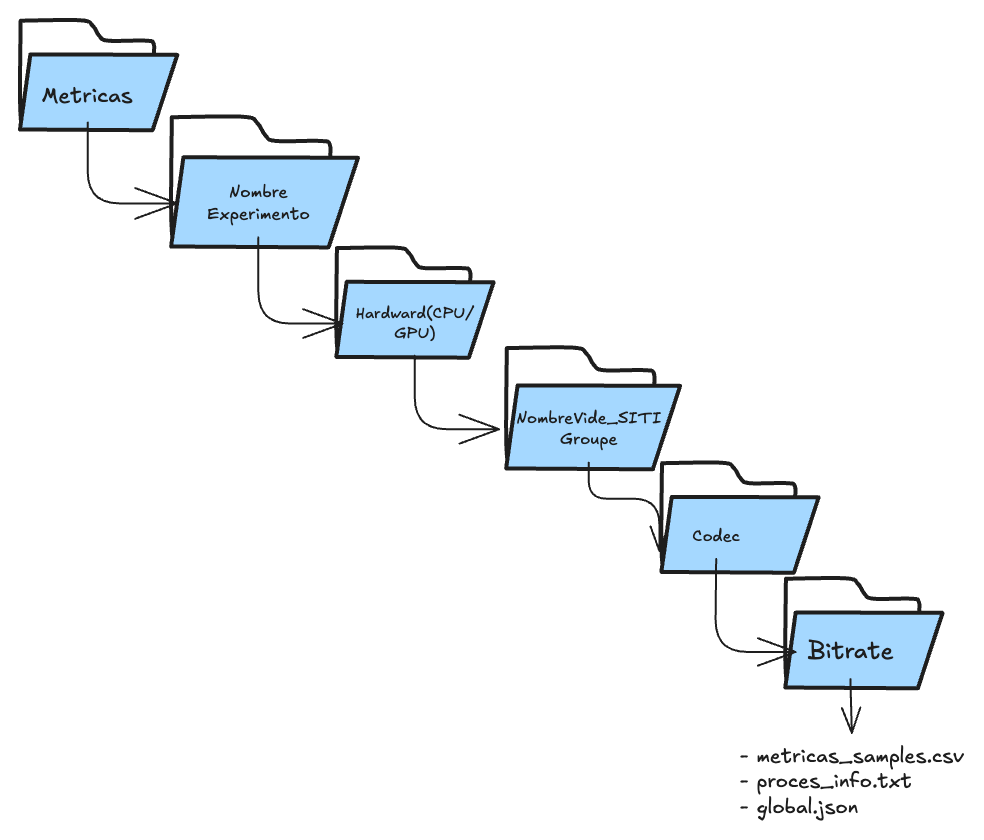
\includegraphics[width=0.3\linewidth]{figs/exp2.1-DataPathSITI.png}

    \caption{Árbol de directorios en el que se almacenan los datos de consumo energéticos de cada iteración}

    \label{fig:exp2.2-datapath}

\end{figure}

%POST-PROCESAMIENTO DATOS

El postprocesamiento de las métricas recopiladas se realizó mediante el script de Python \textbf{ploter-exp2.2.py} (Apéndice\ref{code:exp2.2-ploter} y \ref{code:exp2.2-ploter-obj}). Este script permite procesar y estructurar los datos obtenidos, almacenándolos en un archivo CSV con la estructura mostrada en \ref{fig:exp2.2-csvheader-dataprocess}. Asimismo, permite generar diferentes representaciones gráficas a partir de los datos procesados.

El script está diseñado para ejecutarse desde la interfaz de línea de comandos (\textit{CLI}), mediante diferentes \textit{flags} que permiten especificar tanto el tipo de procesamiento que se desea realizar como la ubicación de los datos de entrada \footnote{Ejecución básica del script \textbf{ploter-exp2.2.py} \lstinline[language=sh]{python3 ploter-exp2.2.py NOMBRE-EXPERIMENTO [FLAGS]}}. Las opciones que acepta el script (tanto opcionales como obligatorias) pueden apreciarse a continuación: 

\begin{itemize}
     \item \textbf{process}: Permite procesar las métricas de consumo obtenidas durante el experimento \textit{exp2.2}. Por defecto, el script accede al directorio \textit{AllMetrics}, aunque es posible especificar una ruta alternativa.

     \item \textbf{plot3d}: Permite representar la posición de cada vídeo en un gráfico tridimensional, en el que el eje X representa el valor de TI, el eje Y el valor de SI y el eje Z el consumo energético del contenedor. Se genera una gráfica para cada combinación de codificador y \textit{bitrate}.

     \item \textbf{plot-consumo-ti}: Permite generar una gráfica bidimensional de tipo \textit{stream} para cada combinación de codificador y \textit{bitrate}. En este caso, el eje X representa el valor de TI y el eje Y el consumo energético, expresado en julios, del proceso de transcodificación.

     \item \textbf{plot-consumo-si}: Permite generar una gráfica bidimensional de tipo \textit{stream} para cada combinación de codificador y \textit{bitrate}. En este caso, el eje X representa el valor de SI y el eje Y el consumo energético, expresado en julios, del proceso de transcodificación.
     
     \item \textbf{plot-consumoxtiempo-grupal}: Permite generar una gráfica de dispersión de puntos, los cuales se agrupan por codec y bitrate utilizado. En este caso lleva a cabo una comparativa entre consumo energético y tiempo de codificación, permitiendo discernir cómo afectan las características de los videos.

     \item \textbf{--data-final-dir=PATH\_ARCHIVO}: Permite definir una ruta alternativa para almacenar el archivo CSV resultante del procesamiento de los datos. Por defecto, se utiliza la ruta \textit{./data/ex2.2\_process\_data.csv}.

     \item \textbf{--container=consumo\_container0\_j}: Permite seleccionar el contenedor cuyos datos de consumo se utilizarán para generar las gráficas, en caso de que se hayan ejecutado varios contenedores. Por defecto, se utilizan los datos correspondientes a la columna \textit{consumo\_container0\_j}.

\end{itemize}

\subsection{Resultados del Experimento 2: Consumo energético en relación al SITI}\label{subsec:exp2.2-siti}
 Los resultados obtenidos durante la fase experimental \textbf{Experimento 2.2: Consumo energético en relación al SITI} \ref{section:exp2.2-sitixconsumo} han permitido analizar la relación existente entre el consumo energético del proceso de transcodificación, las características del contenido de vídeo, representadas mediante las características de vídeo \textit{Spatial Information} (SI) y \textit{Temporal Information} (TI), y el comportamiento de los diferentes codificadores evaluados. Las gráficas utilizadas para este análisis han sido generadas mediante el script de Python \textbf{ploter-exp2.2}, a partir de las métricas obtenidas por el script en Bash \textbf{exp2.2-sisti-energy}. Debido al elevado número de gráficas generadas, se ha incluido en la Figura \ref{fig:resul-exp2} una muestra de los tipos de gráficas obtenidas, habiendo ubicado el resto de figuras en el apartado \textit{Experimento 2.2: Consumo Energético en relación con el SITI} \ref{apendice:exp2.2-graficas} ubicado en el Apéndice.

 En primer lugar, se observa una tendencia general de incremento del consumo energético a medida que aumenta el \textit{bitrate} utilizado durante la codificación. Sin embargo, desde un criterio subjetivo de calidad visual, no se aprecian mejoras significativas a partir de los \textbf{35 Mbps} para los codificadores \textbf{libx264} y \textbf{H264\_NVENC}, ni a partir de los \textbf{30 Mbps} para \textbf{libx265} y \textbf{HEVC\_NVENC}. Este resultado indica que, para los vídeos y condiciones evaluados, incrementar el bitrate por encima de dichos valores supone un aumento del consumo energético sin que dicho incremento se traduzca en una mejora perceptible de la calidad. Por tanto, estos valores podrían considerarse como referencias iniciales para establecer configuraciones de codificación que busquen un compromiso entre calidad visual y eficiencia energética.
 
% ----x264
 En relación con las características SI y TI, los resultados muestran un comportamiento diferente en función del codificador utilizado. Para \textit{libx264} se observa cierta influencia de la componente temporal (\textit{TI}) sobre el consumo energético, aunque la variabilidad existente entre los diferentes vídeos impide establecer una relación directa y concluyente. Esta tendencia puede observarse en las gráficas de consumo energético frente a TI y SI, representadas respectivamente en las Figuras \ref{fig:exp2.2-consumoxsi-libx264-30} y \ref{fig:exp2.2-consumoxti-libx264-30}. Destacar que también se ha observado cierta influencia del \textit{TI} en el tiempo de codificación, de forma que un mayor valor de TI aumenta el tiempo necesario de codificación \ref{fig:exp2.2-consumoxtiempo-group-libx264-30-group}.
% --- x265
 
 El codificador \textbf{libx265} muestra, un mayor consumo energético en los vídeos pertenecientes a las zonas \textbf{HTI\_LSI} y \textbf{LTI\_LSI}. No obstante, estos resultados no permiten establecer una correlación directa entre los valores de SI y TI y el consumo energético. Incluso dentro de un mismo grupo de vídeos, se observa una variabilidad considerable en el consumo, mientras que determinados vídeos pertenecientes a zonas diferentes presentan valores similares. Esto sugiere que el consumo energético del proceso de codificación no depende exclusivamente de las características SI y TI, sino que puede estar condicionado por otras características del contenido y por la configuración interna del propio codificador.

 Al compara los codificadores basados en CPU, el codificador \textbf{libx265} destaca un elevado incremento del consumo energético respecto a \textbf{libx264}. Empleando de base las características del video \textit{IndorSoccer\_0046} codificado a \textbf{40 Mbps} (uno de los videos con mayor consumo energético y el valor máximo de bitrate para la estándar H.265) se observa que el consumo energético experimenta un incremento aproximado del \textbf{$9619,80\%$} respecto al codificador libx264. Asimismo, el tiempo de codificación aumenta entre un \textbf{$70,25\%$} y un \textbf{$74\%$} respecto al tiempo medio observado para libx264.

 % CODIFICACION CON GPU
 En cuanto a los codificadores basados en GPU, el codificador \textbf{H264} muestra una tendencia hacia un mayor consumo energético en aquellos vídeos caracterizados por valores elevados de \textit{SI}. En consecuencia, las zonas \textbf{HSI\_LTI} y \textbf{HSI\_HTI} concentran los vídeos con mayores consumos energéticos, seguidas por \textit{LSI\_HTI}, mientras que los vídeos pertenecientes a \textit{LSI\_LTI} presentan, en términos generales, los menores consumos, pero los tiempos de codificación más elevados. Este comportamiento apunta a una mayor influencia de la complejidad espacial en el consumo energético, así como dificultades para codificar videos con baja información espacial y temporal. Aunque para poder reafirmar este comportamiento, sería necesario disponer de un conjunto de muestras mayor para determinar si esta tendencia puede generalizarse.

 En cuanto a \textbf{HEVC\_NVENC}, en relación al consumo energético y las características SI y TI, los resultados muestran una mayor presencia de consumos elevados en vídeos caracterizados por valores \textit{elevados de SI} y valores \textit{elevados de TI} en el aspecto de consumo energético. Por otra parte, se puede apreciar una fuerte influencia en el ámbito temporal en videos cuyas características presentan valores bajos de SI y TI (\textit{LTI\_LSI}), así como valores altos de TI y bajos en SI (\textit{HTI\_LSI}). Este comportamiento podría indicar que tanto la complejidad temporal como la espacial pueden contribuir al incremento de la carga de codificación, aunque su influencia no puede considerarse independiente a partir de los resultados obtenidos.
 
 % --- GPU vs GPU
 Al comparar ambos codificadores, se aprecia en el codificador \textbf{HEVC\_NVENC} un incremento global del consumo energético del \textit{18,80\%} respecto a \textbf{H264\_NVENC}, acompañado de un incremento del \textit{6,45\%} en los tiempos de codificación. Por tanto, aunque la aceleración mediante GPU permite reducir considerablemente el coste respecto a las alternativas basadas en CPU, la utilización de HEVC continúa suponiendo un coste adicional frente a H.264 en las condiciones analizadas.
 
 % -- GPU VS CPU
 En cuanto a los codificadores que hacen uso de la GPU, \textbf{H264\_NVENC} y \textbf{HEVC\_NVENC}, se observa una reducción general tanto del consumo energético como de los tiempos de codificación respecto a sus equivalentes basados en CPU (\textit{libx264 y libx265}). Utilizando como base la media de los resultados de cada proceso de codificación con cada bitrate, se observa que, al comparar el codificador \textit{h264\_nvenv} frente al codificador \textit{libx264}, el consumo energético se reduce un $70\%-80\%$, al igual que el tiempo de codificación, el cual se reduce entre un $66\%$ y un $71\%$. En el caso del estándar \textit{H.265}, se observan reducciones del consumo energético del $99,53\%-99,67\%$ y reducciones de tiempo de codificación del $86,47\%-99,67\%$ al utilizar el codificador \textit{hevc\_nvenc} frente al codificador \textit{libx265}. Estos resultados ponen de manifiesto el potencial de la aceleración hardware como estrategia para reducir el coste energético asociado a procesos de transcodificación, especialmente cuando se emplean codificadores con una mayor complejidad computacional.

 Un resultado adicional de interés se obtiene al analizar los vídeos construidos a partir de varios \textit{chunks} consecutivos. Estos presentan, en términos generales, un menor consumo energético que el esperado a partir de los \textit{chunks} individuales que los componen. Este comportamiento podría estar relacionado con la reducción del número de cambios de escena y con una mayor eficiencia del proceso de codificación al trabajar sobre una secuencia continua de imágenes. Además, el consumo medio de estos vídeos tiende a situarse por debajo del consumo registrado individualmente en algunos de los \textit{chunks} que los conforman. No obstante, esta observación debe considerarse como una primera indicación y no como una conclusión definitiva, ya que sería necesario ampliar el número de vídeos de este tipo e incrementar la diversidad de contenidos para determinar si existe una relación sistemática entre la continuidad temporal de la secuencia y la eficiencia energética de la codificación.

 \begin{figure}[H]
   \dosubfigs
        {figs/exp2.2/ploter2.2/plot3d/consumo_container0_j-libx264-30_ConsumoSITI.png}{Consumo energético frente a Si y TI codificado con libx264 a 30 Mbps}{fig:exp2.2-plot3d-libx264-30}
        {figs/exp2.2/ploter2.2/consumo-si/consumo_container0_j-libx264-30_ConsumoSI.png}{Consumo energético frente a SI codificado con libx264 a 30 Mbps}{fig:exp2.2-consumoxti-libx264-30}

  \dosubfigs
        {figs/exp2.2/ploter2.2/consumo-ti/consumo_container0_j-libx264-30_ConsumoTI.png}{Consumo energético frente a TI codificado con libx264 a 30 Mbps}{fig:exp2.2-consumoxsi-libx264-30}
        {figs/exp2.2/ploter2.2/consumoxtiempo-group/30/libx264-30_ConsumoxTiempoGroup.png}{Consumo energético frente a tiempo de codificación con libx264 a 30 Mbps}{fig:exp2.2-consumoxtiempo-group-libx264-30-group}
 \caption{Muestra de los tipos de gráficas obtenidas en el Experimento 2}
 \label{fig:resul-exp2}
\end{figure}